\documentclass{article}
\usepackage[english,russian]{babel}
\usepackage{textcomp}
\usepackage{geometry}
  \geometry{left=2cm}
  \geometry{right=1.5cm}
  \geometry{top=1.5cm}
  \geometry{bottom=2cm}
\usepackage{tikz}
\usepackage{multicol}
\usepackage{hyperref}
\usepackage{listings}
\pagenumbering{gobble}

\lstdefinestyle{csMiptCppStyle}{
  language=C++,
  basicstyle=\linespread{1.1}\ttfamily,
  columns=fixed,
  fontadjust=true,
  basewidth=0.5em,
  keywordstyle=\color{blue}\bfseries,
  commentstyle=\color{gray},
  texcl=true,
  stringstyle=\ttfamily\color{orange!50!black},
  showstringspaces=false,
  numbersep=5pt,
  numberstyle=\tiny\color{black},
  numberfirstline=true,
  stepnumber=1,      
  numbersep=10pt,
  backgroundcolor=\color{white},
  showstringspaces=false,
  captionpos=b,
  breaklines=true
  breakatwhitespace=true,
  xleftmargin=.2in,
  extendedchars=\true,
  keepspaces = true,
  tabsize=4,
  upquote=true,
}


\lstdefinestyle{csMiptCppLinesStyle}{
  style=csMiptCppStyle,
  frame=lines,
}

\lstdefinestyle{csMiptCppBorderStyle}{
  style=csMiptCppStyle,
  framexleftmargin=5mm, 
  frame=shadowbox, 
  rulesepcolor=\color{gray}
}


\lstdefinestyle{csMiptBash}{
breaklines=true,
frame=tb,
language=bash,
breakatwhitespace=true,
alsoletter={*()"'0123456789.},
alsoother={\{\=\}},
basicstyle={\ttfamily},
keywordstyle={\bfseries},
literate={{=}{{{=}}}1},
prebreak={\textbackslash},
sensitive=true,
stepnumber=1,
tabsize=4,
morekeywords={echo, function},
otherkeywords={-, \{, \}},
literate={\$\{}{{{{\bfseries{}\$\{}}}}2,
upquote=true,
frame=none
}


\lstset{style=csMiptCppStyle}
\lstset{literate={~}{{\raisebox{0.5ex}{\texttildelow}}}{1}}


\renewcommand{\thesubsection}{\arabic{subsection}}
\makeatletter
\def\@seccntformat#1{\@ifundefined{#1@cntformat}%
   {\csname the#1\endcsname\quad}
   {\csname #1@cntformat\endcsname}}
\newcommand\section@cntformat{}     
\newcommand\subsection@cntformat{Задача \thesubsection.\space} 
\newcommand\subsubsection@cntformat{\thesubsubsection.\space}
\makeatother



\begin{document}
\title{Семинар \#1: Основы git. Практика. \vspace{-5ex}}\date{}\maketitle

\subsection{Hello}
Напишите \texttt{bash}-скрипт, который должен делать следующее:
\begin{enumerate}
\item Писать на экране сообщение \texttt{Hello World!}.
\item Создавать файл \texttt{hello.txt}, в котором будет записано \texttt{Hello World!}.
\end{enumerate}
Протестируйте ваш \texttt{bash}-скрипт, запустив его.


\subsection{Создайте папку с файлами}
Напишите \texttt{bash}-скрипт, который должен делать следующее:
\begin{enumerate}
\item Создавать папку \texttt{animals} в текущей директории.
\item В этой папке создавать 2 файла: \texttt{cat.txt} и \texttt{dog.txt}.
\item В файл \texttt{cat.txt} нужно записать строку \texttt{"I am Cat!"}, а в файл \texttt{dog.txt} записать строку \texttt{"I am Dog!"}.
\item После исполнения скрипта в \texttt{bash} пользователь должен остаться в той же директории, в которой скрипт был запущен.
\item Писать сообщение об успешном завершении.
\end{enumerate}
Протестируйте ваш \texttt{bash}-скрипт, запустив его.


\subsection{Репозиторий из четырёх коммитов}
\begin{minipage}{0.5\linewidth}
Напишите \texttt{bash}-скрипт, который должен делать следующее:
\begin{enumerate}
\item Инициализировать новый пустой git репозиторий.
\item Создавать новый файл \texttt{cat.txt} и добавлять коммит в репозиторий, содержащий этот файл.
\item Создавать новый файл \texttt{dog.txt} и добавлять коммит, содержащий файл \texttt{dog.txt}.
\item Изменять файл \texttt{cat.txt} и добавлять коммит, содержащий эти изменения.
\item Удалять файл \texttt{dog.txt} и добавлять коммит, который уже не содержит файл \texttt{dog.txt}.
\item Сообщения коммитов должны корректно описывать происходящее.
\item Печатать информацию о всех сделанных коммитах в следующем формате:
\begin{lstlisting}[style=csMiptBash]
$ git log --oneline --all --graph
\end{lstlisting}
\end{enumerate}
Протестируйте ваш \texttt{bash}-скрипт, запустив его.
\end{minipage}
\begin{minipage}{0.4\linewidth}
\begin{center}
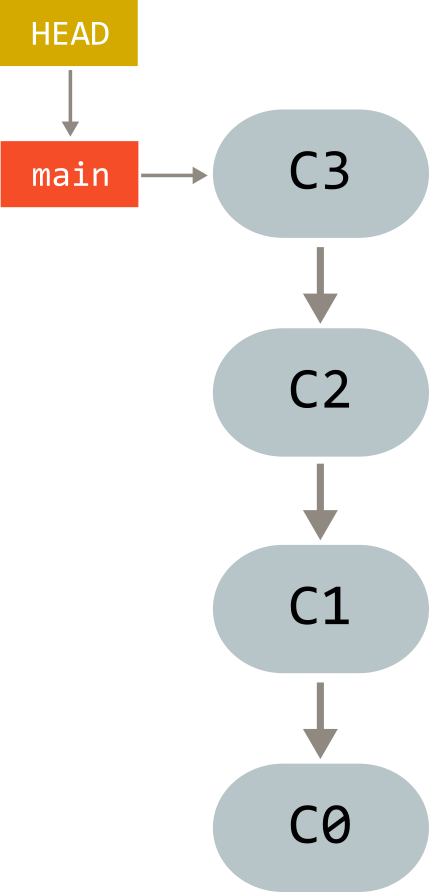
\includegraphics[scale=1]{../images/four_commits.png}
\end{center}
\end{minipage}


\newpage
\subsection{Две ветки}
Создайте новый локальный репозиторий и добавьте в него коммиты, таким образом, чтобы граф коммитов выглядел так, как это представлено на рисунке:
\begin{center}
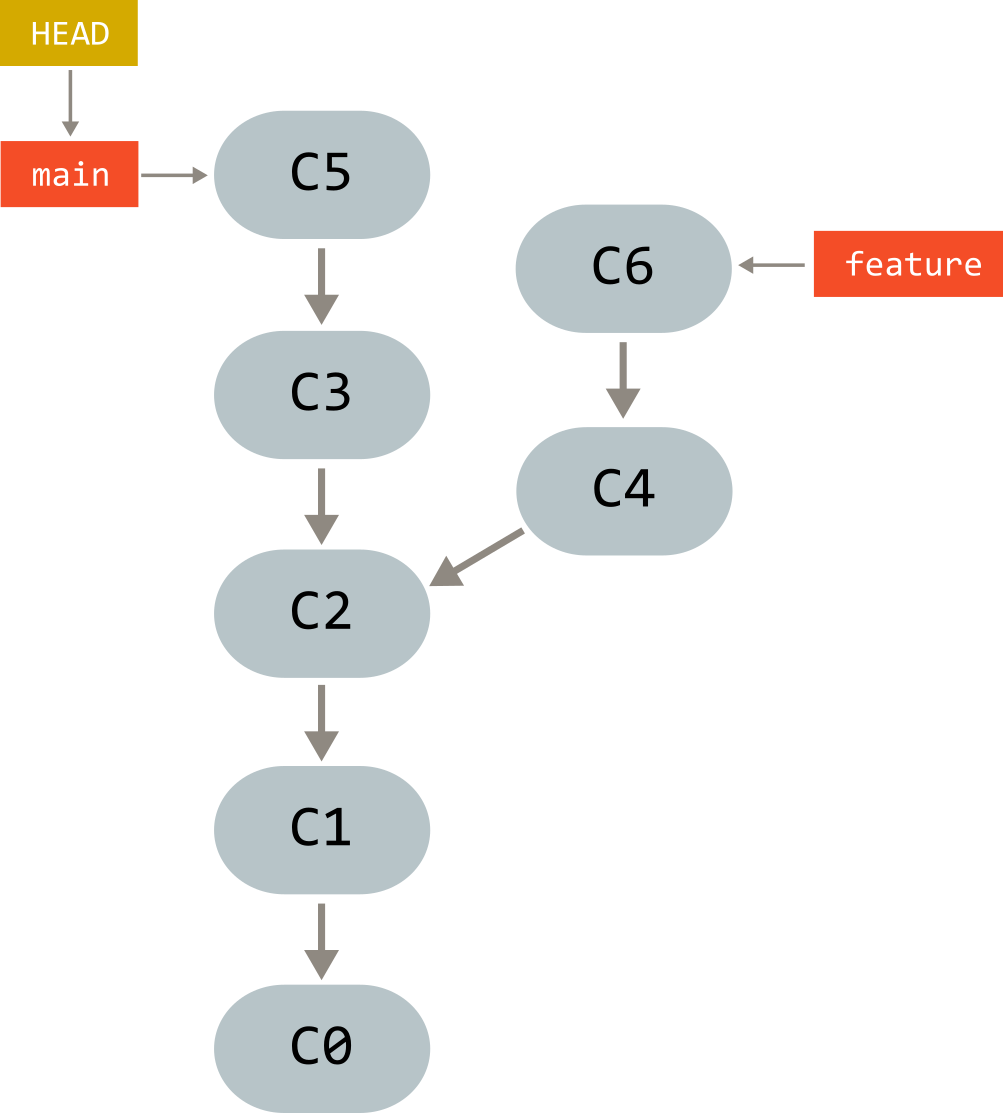
\includegraphics[scale=0.9]{../images/two_branches.png}
\end{center}
В репозитории должно быть две ветки: \texttt{main} и \texttt{feature}. Порядок добавления коммитов должен соответствовать порядковым номерам, изображенным на рисунке. Сообщения коммитов должны начинаться на их обозначения, изображенным на рисунке (\texttt{C0}, \texttt{С1} и т. д.). Конкретное содержимое файлов репозитория может быть любым -- на ваш выбор. Для просмотра графа коммитов используйте:
\begin{lstlisting}[style=csMiptBash]
$ git log --oneline --all --graph
\end{lstlisting}
Создайте bash-скрипт, который бы содержал все команды из этого задания (он должен с нуля создавать репозиторий, представленный на изображении). Протестируйте этот bash-скрипт.


\subsection{Граф со слияниями}
Сделать всё то же самое, что и в предыдущей задаче, но граф коммитов должен выглядеть так:
\begin{center}
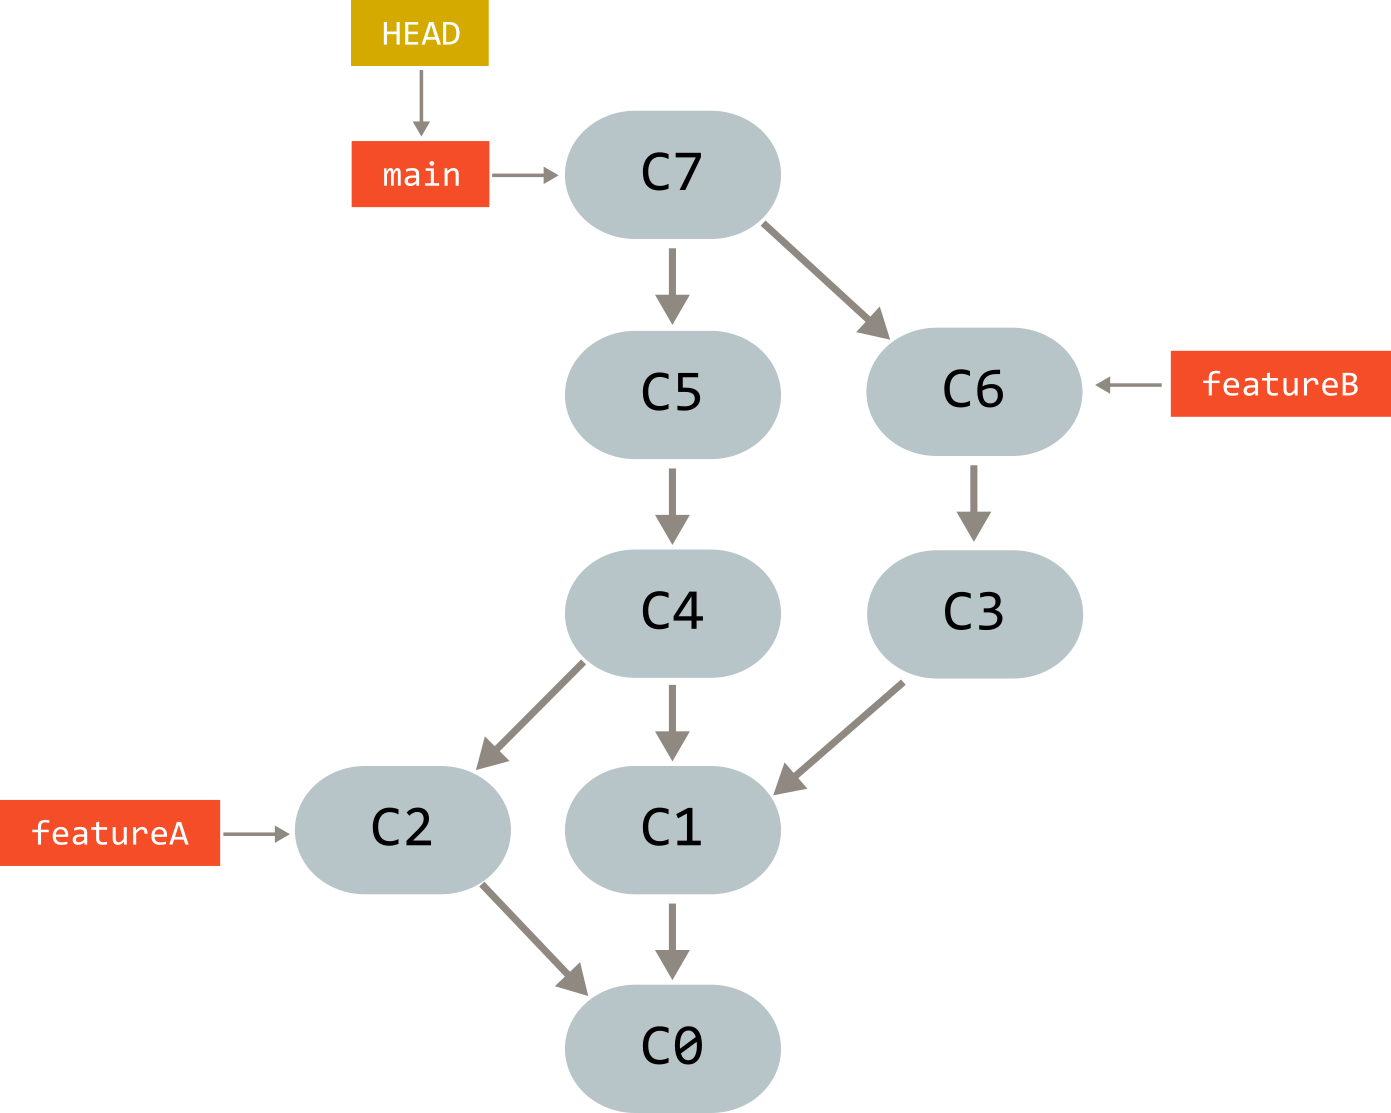
\includegraphics[scale=0.9]{../images/graph_with_merges.png}
\end{center}
После этого удалите ветки \texttt{featureA} и \texttt{featureB} отдельными командами.


\subsection{Слияние с конфликтом}
Для проверки числа на простоту на языке C была написана функция \texttt{is\_prime}. Эта функция находится в файле \texttt{prime.c} в репозитории \href{https://mipt-hsse.gitlab.yandexcloud.net/v.biryukov/prime_calculation}{\texttt{mipt-hsse.gitlab.yandexcloud.net/v.biryukov/prime\_calculation}}. В какой-то момент файл \texttt{prime.c} выглядел следующим образом:
\begin{lstlisting}
#include <stdio.h>

int is_prime(int n)
{
    if (n < 2) 
        return 0;

    for (int i = 2; i < n; ++i)
    {
        if (n % i == 0)
            return 0;
    }
    return 1;
}

int main()
{
    int a = 25263551;

    if (is_prime(a))
        printf("%i is prime\n", a);
    else
        printf("%i is NOT prime\n", a);
}
\end{lstlisting}
Над этим проектом работала команда программистов, и в определённый момент практически одновременно произошли следующие события:
\begin{itemize}
\item Программист Алиса заметила, что алгоритм проверки числа на простоту не оптимален и его можно ускорить, если производить итерации не до $n$, а до $\sqrt{n}$. Алиса создала новую ветку \texttt{alice} и добавила в него коммит, с такой оптимизацией.
\item В это же самое время программист Боб заметил, что алгоритм можно ускорить, если в процессе итерирования пропускать чётные числа (однако Боб не заметил оптимизацию, которую заметила Алиса). Боб создал новую ветку \texttt{bob} и добавил в него коммит, со своей оптимизацией.
\item Параллельно с этим другие участники команды продолжали развивать проект. В главной ветке \texttt{main} появился новый коммит, расширяющий набор тестов в функции \texttt{main}.
\end{itemize}
Ваша задача -- объединить все изменения из веток \texttt{alice} и \texttt{bob} в ветку \texttt{main}. После успешного объединения необходимо удалить ветки \texttt{alice} и \texttt{bob}.
Затем нужно создать репозиторий на GitLab и отправить туда ваш репозиторий.
\\[5mm]
\noindent Решите эту задачу двумя способами:
\begin{enumerate}
\item Используя слияние -- \texttt{git merge}.
\item Используя перебазирование -- \texttt{git rebase}.
\end{enumerate}
То есть в итоге на GitLab нужно будет создать 2 репозитория \texttt{prime\_calculation\_merge} и \texttt{prime\_calculation\_rebase}. В одном будет результат выполнения задания с помощью \texttt{git merge}, а в другом -- с помощью \texttt{git rebase}.

Граф репозитория можно посмотреть на GitLab, если на странице репозитория нажать на левой панели \texttt{Code -> Repository graph}.



\iffalse
После выполнения задания вам нужно создать файл с помощью команды:
\begin{lstlisting}[style=csMiptBash]
$ git log -p --all > result_merge.txt      # после решении задачи с помощью git merge
$ git log -p --all > result_rebase.txt     # после решении
Эти файлы нужно будет закомитить в ваш репозиторий с домашними заданиями. задачи с помощью git rebase
\end{lstlisting}
\fi

\subsection{HEAD}
Напишите bash-скрипт, который бы создавал новый git-репозиторий и приводил бы его в состояние \texttt{detached HEAD}.

\subsection{Просмотр репозитория библиотеки stb}
STB -- это набор header-only библиотек на C/C++, распространяемых в виде исходного кода. Библиотека предоставляет минималистичные решения для распространённых задач: загрузки и сохранения изображений в разных форматах (\texttt{.jpg}, \texttt{.png} и другие), работы со шрифтами, декодирования аудио и обработки данных. Её ключевые преимущества -- простота интеграции, отсутствие внешних зависимостей и удобство использования. STB идеально подходит для быстрого прототипирования, небольших проектов и сценариев, где не требуются сложные специализированные библиотеки.

Репозиторий проекта можно найти на GitHub: \href{https://github.com/nothings/stb}{\texttt{github.com/nothings/stb}}. Вам нужно клонировать этот репозиторий себе и произвести следующие операции:

\begin{enumerate}
\item Просмотрите всю историю коммитов с помощью команды:
\begin{lstlisting}[style=csMiptBash]
$ git log --oneline --all --graph
\end{lstlisting}
Удобнее смотреть в файле:
\begin{lstlisting}[style=csMiptBash]
$ git log --oneline --all --graph > history.txt
\end{lstlisting}
\item Выполните команду, которая бы печатала информацию о всех коммитах, сделанных с начала текущего года.
\item Выполните команду, которая бы печатала информацию о всех коммитах, в которых менялся файл \texttt{stb\_image.h}.
\item Выполните команду, которая бы печатала информацию о всех коммитах, в которых изменялась функция \texttt{stbi\_jpeg\_load} из файла \texttt{stb\_image.h}.
\item Используйте \texttt{git switch}, чтобы перейти на второй коммит в истории проекта. Создайте новую ветку, указывающую на этот коммит.
\item Используйте \texttt{git rebase} чтобы "выпрямить"{} историю коммитов.
\item Используйте интерактивный \texttt{git rebase} чтобы сжать всю историю до 10-ти коммитов. Выберете коммиты равномерно в истории проекта. 
\end{enumerate}



\subsection{Задание совместную работу с репозиторием}
Сделайте задание по адресу  \texttt{\href{https://mipt-hsse.gitlab.yandexcloud.net/pro100savant/hellow_word_2025}{mipt-hsse.gitlab.yandexcloud.net/pro100savant/hellow\_word\_2025}}.


\end{document}
